% Compile with: tectonic main.tex   (or pdflatex / Overleaf)
\documentclass[11pt,aspectratio=169]{beamer}

\title{Identifiability Guarantees for Causal Disentanglement from Soft Interventions}
\date[Seminar talk]{Zhang et al.\ (2023), with von K\"ugelgen et al.\ (2023)}
\author{Joan and Francesco} % TODO: full names
\institute{ETH Zurich}

\usetheme{eth}

\colorlet{titlefgcolor}{ETHBlue}
\colorlet{accentcolor}{ETHBlue}

\usetikzlibrary{arrows.meta,positioning,shapes.geometric,fit,calc}
\tikzset{
  lat/.style={circle,draw,minimum size=7mm,inner sep=0pt,font=\footnotesize},
  intv/.style={lat,draw=ETHRed,very thick,text=ETHRed},
  arr/.style={-{Stealth[length=2mm]},thick},
  gone/.style={-{Stealth[length=2mm]},thick,dashed,draw=black!30},
  lbl/.style={font=\scriptsize,align=center},
}

\newcommand{\PP}{\mathbb{P}}
\newcommand{\pa}{\mathrm{pa}}
\newcommand{\G}{\mathcal{G}}
\newcommand{\D}{\mathcal{D}}
\newcommand{\red}[1]{\textcolor{ETHRed}{#1}}
\newcommand{\src}[1]{\par\vfill{\tiny\textcolor{ETHGray}{#1}}}
\newcommand{\crl}{\sim_{\textsc{crl}}}

\begin{document}

\setlength{\titleboxwidth}{0.5\textwidth}
\titleframe

%======================================================================
\section{Introduction \hfill {\normalsize Joan}}
%======================================================================

\begin{frame}{The variables we measure are rarely the causal ones}
	\begin{columns}[onlytextwidth,t]
		\begin{column}{0.47\textwidth}
			\begin{block}{Images}
				\begin{itemize}
					\item Pixel $i$ in one image has no relation to pixel $i$ in another.
					\item Intervening on a single pixel means nothing.
					\item The causal variables are \emph{objects}: abstract functions of pixels.
				\end{itemize}
			\end{block}
		\end{column}
		\begin{column}{0.47\textwidth}
			\begin{block}{Gene expression}
				\begin{itemize}
					\item More than 20{,}000 human genes are measured per cell.
					\item Genes in the same pathway act together.
					\item The causal variables are \emph{programs}: groups of genes.
				\end{itemize}
			\end{block}
		\end{column}
	\end{columns}
	\bigskip
	Classical causal structure learning assumes that the causal variables are observed.\\[1mm]
	Here they are not: \alert{the causal variables have to be learned}.
\end{frame}

\begin{frame}{Causal disentanglement}
	\framesubtitle{Also called causal representation learning}
	\begin{columns}[onlytextwidth]
		\begin{column}{0.52\textwidth}
			\centering
			\begin{tikzpicture}[node distance=6mm and 7mm]
				\node[lat] (u1) {$U_1$};
				\node[lat,below left=of u1] (u2) {$U_2$};
				\node[lat,below right=of u1] (u4) {$U_4$};
				\node[lat,below right=of u2] (u3) {$U_3$};
				\draw[arr] (u1) -- (u2); \draw[arr] (u1) -- (u4); \draw[arr] (u2) -- (u3); \draw[arr] (u2) -- (u4);
				\node[draw,dashed,rounded corners,fit=(u1)(u2)(u3)(u4),inner sep=2mm,label={[lbl]above:latent DAG $\G$}] (box) {};
				\node[trapezium,draw,fill=ETHBlue!15,shape border rotate=270,minimum height=8mm,minimum width=16mm,right=6mm of box] (f) {$f$};
				\node[draw,fill=ETHGray!15,minimum width=12mm,minimum height=22mm,right=6mm of f,label={[lbl]above:observed $X$}] (x) {};
				\foreach \y in {-8,-4,0,4,8} \draw[ETHGray!60] ($(x.west)+(0,\y mm)$) -- ($(x.east)+(0,\y mm)$);
				\draw[arr] (box) -- (f); \draw[arr] (f) -- (x);
			\end{tikzpicture}
		\end{column}
		\begin{column}{0.46\textwidth}
			\begin{itemize}
				\item A few latent variables $U$, related by an unknown DAG $\G$.
				\item An unknown mixing function $f$ maps them to what we observe.
				\item Goal: recover the latent variables \emph{and} their causal graph from samples of $X$ only.
			\end{itemize}
		\end{column}
	\end{columns}
\end{frame}

\begin{frame}{Why interventions: single-cell perturbation screens}
	\begin{itemize}
		\item CRISPR screens (Perturb-seq) perturb one or several genes and read out the expression of every cell.
		\item This gives one dataset per perturbation, next to the unperturbed cells.
		\item Sequencing destroys the cell, so each cell is seen under \emph{one} condition only: the data are \alert{unpaired}.
		\item A CRISPR activation does not fix a gene to a value. It changes how the gene responds to its regulators: a \alert{soft} intervention.
	\end{itemize}
	\bigskip
	\begin{block}{What we want in the end}
		Find the gene programs and how they regulate each other, and predict the effect of perturbation \emph{combinations} that were never measured.
	\end{block}
\end{frame}

\begin{frame}{Two papers, one question}
	\begin{block}{Question}
		When do interventions make the latent causal model identifiable, and how do we learn it in practice?
	\end{block}
	\medskip
	\begin{columns}[onlytextwidth,t]
		\begin{column}{0.47\textwidth}
			\textbf{Additional paper}\\
			von K\"ugelgen et al., \emph{Nonparametric Identifiability of Causal Representations from Unknown Interventions}, 2023
			\begin{itemize}
				\item No assumption on the mixing or the mechanisms.
				\item Needs \emph{hard} interventions.
			\end{itemize}
		\end{column}
		\begin{column}{0.47\textwidth}
			\textbf{Main paper}\\
			Zhang et al., \emph{Identifiability Guarantees for Causal Disentanglement from Soft Interventions}, 2023
			\begin{itemize}
				\item Polynomial mixing.
				\item Works with \emph{soft} interventions, and comes with an algorithm.
			\end{itemize}
		\end{column}
	\end{columns}
\end{frame}

%======================================================================
\section{Problem setup \hfill {\normalsize Joan}}
%======================================================================

\begin{frame}{Data-generating process}
	\[
		X = f(U), \qquad U \sim \PP_U = \prod_{i=1}^{p} \PP\big(U_i \mid U_{\pa_\G(i)}\big)
	\]
	\begin{itemize}
		\item $X = (X_1,\dots,X_n)$: observed variables, e.g.\ the expression of $n$ genes.
		\item $U = (U_1,\dots,U_p)$: latent causal variables, with $p \ll n$ in practice.
		\item $\G$: unknown DAG on $\{1,\dots,p\}$; $\PP_U$ factorizes according to $\G$.
		\item $f$: unknown deterministic mixing function, possibly non-linear.
	\end{itemize}
	\bigskip
	\begin{block}{Unknown}
		The latent variables $U$, their number $p$, the graph $\G$, the mixing $f$, and which latent each intervention targets.
	\end{block}
\end{frame}

\begin{frame}{What does ``identifiable'' mean?}
	\begin{itemize}
		\item A latent model is \alert{identifiable} if it is the only one that explains the distribution of the data.
		\item All statements are for the infinite-data regime: the distributions of $X$ are known exactly.
		\item Uniqueness is never literal. Two changes can always be absorbed by the mixing $f$:
		\begin{itemize}
			\item relabeling the latent variables (a permutation);
			\item rescaling each latent variable.
		\end{itemize}
		\item So the best possible result is identifiability \alert{up to an equivalence class}.
	\end{itemize}
	\bigskip
	The two papers differ in how large this class is, and in what they assume to reach it.
\end{frame}

%======================================================================
\section{Setup shared by both papers \hfill {\normalsize Francesco}}
%======================================================================

\begin{frame}{Hard and soft interventions}
	An intervention $I$ with target $i$ changes one conditional $\PP(U_i \mid U_{\pa(i)})$ and leaves all others untouched.
	\medskip
	\begin{center}
	\begin{tikzpicture}
		\begin{scope}
			\node[lat] (a) {$U_1$}; \node[lat,right=12mm of a] (b) {$U_2$};
			\draw[arr] (a) -- (b);
			\node[lbl,above=5mm of $(a)!0.5!(b)$] {\textbf{Observational}};
			\node[lbl,below=5mm of $(a)!0.5!(b)$] {$\PP(U_2 \mid U_1)$};
		\end{scope}
		\begin{scope}[xshift=45mm]
			\node[lat] (a) {$U_1$}; \node[intv,right=12mm of a] (b) {$U_2$};
			\draw[gone] (a) -- (b);
			\node[lbl,above=5mm of $(a)!0.5!(b)$] {\textbf{Hard} (perfect)};
			\node[lbl,below=5mm of $(a)!0.5!(b)$] {\red{$\PP^I(U_2)$}};
		\end{scope}
		\begin{scope}[xshift=90mm]
			\node[lat] (a) {$U_1$}; \node[intv,right=12mm of a] (b) {$U_2$};
			\draw[arr] (a) -- (b);
			\node[lbl,above=5mm of $(a)!0.5!(b)$] {\textbf{Soft} (imperfect)};
			\node[lbl,below=5mm of $(a)!0.5!(b)$] {\red{$\PP^I(U_2 \mid U_1)$}};
		\end{scope}
	\end{tikzpicture}
	\end{center}
	\begin{itemize}
		\item \textbf{Hard}: the target no longer depends on its parents.
		\item \textbf{Soft}: the dependence stays, the mechanism changes. Hard is a special case.
		\item Example of a soft intervention, a shift by $a_i$: \quad $\PP^I(U_i = u + a_i \mid U_{\pa(i)}) = \PP(U_i = u \mid U_{\pa(i)})$.
		\item Both papers use \emph{single-node} (atomic) interventions.
	\end{itemize}
\end{frame}

\begin{frame}{The data: unpaired environments with unknown targets}
	\begin{columns}[onlytextwidth]
		\begin{column}{0.56\textwidth}
			We observe samples of $X$ from
			\[
				\D,\ \D^{I_1},\ \dots,\ \D^{I_K}
			\]
			one observational dataset and one per intervention.
			\begin{itemize}
				\item \textbf{Shared}: the mixing $f$ and every mechanism that is not targeted.
				\[
					\PP^{I}_U = \red{\PP^{I}\big(U_i \mid U_{\pa(i)}\big)} \prod_{j \neq i} \PP\big(U_j \mid U_{\pa(j)}\big)
				\]
				\item \textbf{Unpaired}: no sample is seen before \emph{and} after an intervention.
				\item \textbf{Unknown targets}: we know which dataset a sample belongs to, not which latent was changed.
			\end{itemize}
		\end{column}
		\begin{column}{0.4\textwidth}
			\centering
			\begin{tikzpicture}[node distance=4mm]
				\foreach \k/\lab/\col in {0/$\D$/black,1/$\D^{I_1}$/ETHRed,2/$\D^{I_2}$/ETHRed}{
					\begin{scope}[yshift=-\k*17mm]
						\node[lat,minimum size=5.5mm] (a\k) {\tiny$U_1$};
						\node[lat,minimum size=5.5mm,right=6mm of a\k] (b\k) {\tiny$U_2$};
						\draw[arr] (a\k) -- (b\k);
						\node[trapezium,draw,fill=ETHBlue!15,shape border rotate=270,minimum height=5mm,minimum width=9mm,right=5mm of b\k] (f\k) {\scriptsize$f$};
						\node[right=5mm of f\k,font=\scriptsize,text=\col] (x\k) {\lab};
						\draw[arr] (b\k) -- (f\k); \draw[arr] (f\k) -- (x\k);
					\end{scope}
				}
				\node[intv,minimum size=5.5mm] at (a1) {\tiny$U_1$};
				\node[intv,minimum size=5.5mm] at (b2) {\tiny$U_2$};
			\end{tikzpicture}
		\end{column}
	\end{columns}
\end{frame}

\begin{frame}{Faithfulness: the graph can be read from the distribution}
	\begin{columns}[onlytextwidth]
		\begin{column}{0.6\textwidth}
			\begin{itemize}
				\item \textbf{Markov}: every separation in $\G$ gives a conditional independence in $\PP_U$. This is the factorization.
				\item \textbf{Faithfulness}: the converse. The \emph{only} conditional independences in $\PP_U$ are those implied by $\G$.
				\item It excludes exact cancellations. On the right, with $c = -ab$ the two paths cancel and $U_1 \perp\!\!\!\perp U_3$, although $U_1$ causes $U_3$.
				\item Such cancellations need fine-tuned parameters, so faithfulness is a genericity assumption.
			\end{itemize}
		\end{column}
		\begin{column}{0.36\textwidth}
			\centering
			\begin{tikzpicture}[node distance=9mm and 9mm]
				\node[lat] (a) {$U_1$};
				\node[lat,below right=of a] (b) {$U_2$};
				\node[lat,above right=of b] (c) {$U_3$};
				\draw[arr] (a) -- node[lbl,below left=-1mm] {$a$} (b);
				\draw[arr] (b) -- node[lbl,below right=-1mm] {$b$} (c);
				\draw[arr,ETHRed] (a) -- node[lbl,above,text=ETHRed] {$c = -ab$} (c);
			\end{tikzpicture}
		\end{column}
	\end{columns}
	\medskip
	\begin{block}{Role in the two papers}
		\begin{itemize}
			\item von K\"ugelgen et al.: assumed for $\PP_U$; it is what turns ``the latents are recovered'' into ``the graph is recovered''.
			\item Zhang et al.: the same idea, stated for interventions: an intervention must visibly change what is downstream of its target, even after mixing. Details in the second half.
		\end{itemize}
	\end{block}
\end{frame}

\begin{frame}{Why observational data is not enough}
	\begin{enumerate}
		\item \textbf{Even if $U$ were observed}, i.i.d.\ data gives the graph only up to Markov equivalence: $U_1 \to U_2$ and $U_1 \leftarrow U_2$ fit equally well.
		\medskip
		\item \textbf{With an unknown mixing it gets worse.} Write each latent as a function of independent noise, $U = g(\varepsilon)$. Then
		\[
			X = f(U) = (f \circ g)(\varepsilon).
		\]
		Independent latents $\varepsilon$ with the \emph{empty} graph and mixing $f \circ g$ explain the data just as well.
	\end{enumerate}
	\medskip
	\begin{block}{Consequence}
		From observational data alone, any causal DAG can explain the distribution of $X$.
		The causal variables are singled out by what is special about them: \alert{interventions act on them}.
	\end{block}
\end{frame}

\begin{frame}{What is the best we can hope for?}
	Some ambiguity can never be removed, because the mixing $f$ absorbs it.
	\medskip
	\begin{center}
		\begin{tabular}{@{}p{0.3\textwidth}p{0.3\textwidth}p{0.3\textwidth}@{}}
			\toprule
			& von K\"ugelgen et al. & Zhang et al. \\
			\midrule
			Order of the latents & any relabeling $\pi$ & any relabeling $\pi$ \\[1mm]
			Scale of each latent & any invertible map $\phi_i(U_i)$ & affine map $\lambda_i U_i + b_i$ \\[1mm]
			Graph & $\G$ up to relabeling & $\G$ up to relabeling \\
			\bottomrule
		\end{tabular}
	\end{center}
	\medskip
	\begin{itemize}
		\item A result of the form ``the model is identified up to these changes'' is the target in both papers.
		\item The open question is which data and assumptions get us there.
	\end{itemize}
\end{frame}

\begin{frame}{Common ground of the two papers}
	\begin{columns}[onlytextwidth,t]
		\begin{column}{0.47\textwidth}
			\begin{block}{Model}
				\begin{itemize}
					\item Latent variables follow a DAG model: $\PP_U$ factorizes according to $\G$.
					\item Mechanisms are nonparametric.
					\item The mixing $f$ is deterministic, invertible on its image, and the same in all environments.
					\item A faithfulness-type assumption links $\G$ and the distributions.
				\end{itemize}
			\end{block}
		\end{column}
		\begin{column}{0.47\textwidth}
			\begin{block}{Data}
				\begin{itemize}
					\item Several environments, unpaired samples.
					\item Each environment changes \emph{one} mechanism; all others are shared.
					\item Intervention targets are unknown.
					\item Every latent is intervened on at least once.
					\item Results hold for infinite data.
				\end{itemize}
			\end{block}
		\end{column}
	\end{columns}
	\bigskip
	\textbf{Where they differ:} the class of mixing functions, hard versus soft interventions, and whether the number of latents is known.
\end{frame}

%======================================================================
\section{Setup of the additional paper \hfill {\normalsize Francesco}}
%======================================================================

\begin{frame}{Setting: nothing is parametric}
	\framesubtitle{von K\"ugelgen et al., 2023. The paper writes $V$ for the latents; we keep $U$.}
	On top of the common ground:
	\medskip
	\begin{columns}[onlytextwidth,t]
		\begin{column}{0.47\textwidth}
			\begin{block}{More general}
				\begin{itemize}
					\item Latent SCM: $U_i := f_i(U_{\pa(i)}, \varepsilon_i)$, with arbitrary $f_i$ and independent noise.
					\item Mixing $f$: \alert{any} smooth invertible map onto its image.
				\end{itemize}
			\end{block}
		\end{column}
		\begin{column}{0.47\textwidth}
			\begin{block}{More restrictive}
				\begin{itemize}
					\item Interventions are \alert{perfect} (hard).
					\item The number of latents $n$ is known.
				\end{itemize}
			\end{block}
		\end{column}
	\end{columns}
	\bigskip
	Earlier results needed paired counterfactual data, known targets or graph, or linear/polynomial models.\\[1mm]
	\textbf{Question:} are unknown interventions alone enough when both $f$ and the mechanisms are unrestricted?
\end{frame}

\begin{frame}{What does it mean to recover the model?}
	\begin{columns}[onlytextwidth]
		\begin{column}{0.56\textwidth}
			We learn an encoder $Z = h(X)$ and a graph $G'$ on $Z$. Success means:
			\begin{itemize}
				\item every learned $Z_j$ is \emph{one} true latent $U_i$, up to its scale;
				\item the learned graph is the true graph, up to the names of the nodes.
			\end{itemize}
			\medskip
			Two remarks:
			\begin{itemize}
				\item This is the best possible. Interventional data cannot tell two such solutions apart.
				\item Scale is arbitrary, but the \emph{strength} of each arrow is the same in all solutions. The learned graph carries quantitative information.
			\end{itemize}
		\end{column}
		\begin{column}{0.4\textwidth}
			\centering
			\begin{tikzpicture}
				\node[lat] (a) {$U_1$}; \node[lat,right=12mm of a] (b) {$U_2$};
				\draw[arr] (a) -- (b);
				\node[lat,below=14mm of a] (c) {$Z_2$}; \node[lat,right=12mm of c] (d) {$Z_1$};
				\draw[arr] (c) -- (d);
				\draw[dashed,ETHBlue,thick] (a) -- node[lbl,left] {$\phi_1$} (c);
				\draw[dashed,ETHBlue,thick] (b) -- node[lbl,right] {$\phi_2$} (d);
				\node[lbl,left=2mm of a] {truth}; \node[lbl,left=2mm of c] {learned};
			\end{tikzpicture}
		\end{column}
	\end{columns}
\end{frame}

%======================================================================
\section{Additional paper: result and ideas \hfill {\normalsize Francesco}}
%======================================================================

\begin{frame}{Main result: unknown hard interventions are enough}
	\begin{columns}[onlytextwidth,t]
		\begin{column}{0.47\textwidth}
			\begin{block}{Two latents}
				Three datasets suffice: the observational one, and one hard intervention on each latent.\\[1mm]
				Both latents and the direction of the edge are recovered.
			\end{block}
		\end{column}
		\begin{column}{0.47\textwidth}
			\begin{block}{Any number of latents}
				Two different hard interventions on each latent suffice.\\[1mm]
				We must know which two datasets belong together, not which latent they target.
			\end{block}
		\end{column}
	\end{columns}
	\bigskip
	\begin{itemize}
		\item Holds for any mixing and any mechanisms, as long as nothing is fine-tuned.
		\item It is the cause--effect problem, but with unobserved cause and effect.
		\item The pairs are pairs of \emph{datasets}, e.g.\ the same experiment at two doses. Samples stay unpaired.
		\item The authors conjecture that one intervention per latent is enough in general.
	\end{itemize}
\end{frame}

\begin{frame}{Idea 1: compare environments}
	Two environments differ in a single mechanism. Divide their densities: everything shared cancels.
	\[
		\frac{p^{e_1}(u)}{p^{e_0}(u)} = \frac{\red{\tilde p_1(u_1)}\; p_2(u_2 \mid u_1)}{p_1(u_1)\; p_2(u_2 \mid u_1)} = \frac{\red{\tilde p_1(u_1)}}{p_1(u_1)}
	\]
	\begin{itemize}
		\item The ratio depends on \emph{one} variable only: the intervention target.
		\item The learned model must reproduce the same ratio, also as a function of a single learned variable.
		\item This ties one learned variable to one true variable: it cannot be a mixture of several latents.
	\end{itemize}
	\medskip
	\begin{block}{Take-away}
		A sparse change between environments is what separates the latents from each other. No assumption on the shape of $f$ is used.
	\end{block}
\end{frame}

\begin{frame}{The difficulty: targets are unknown}
	\centering
	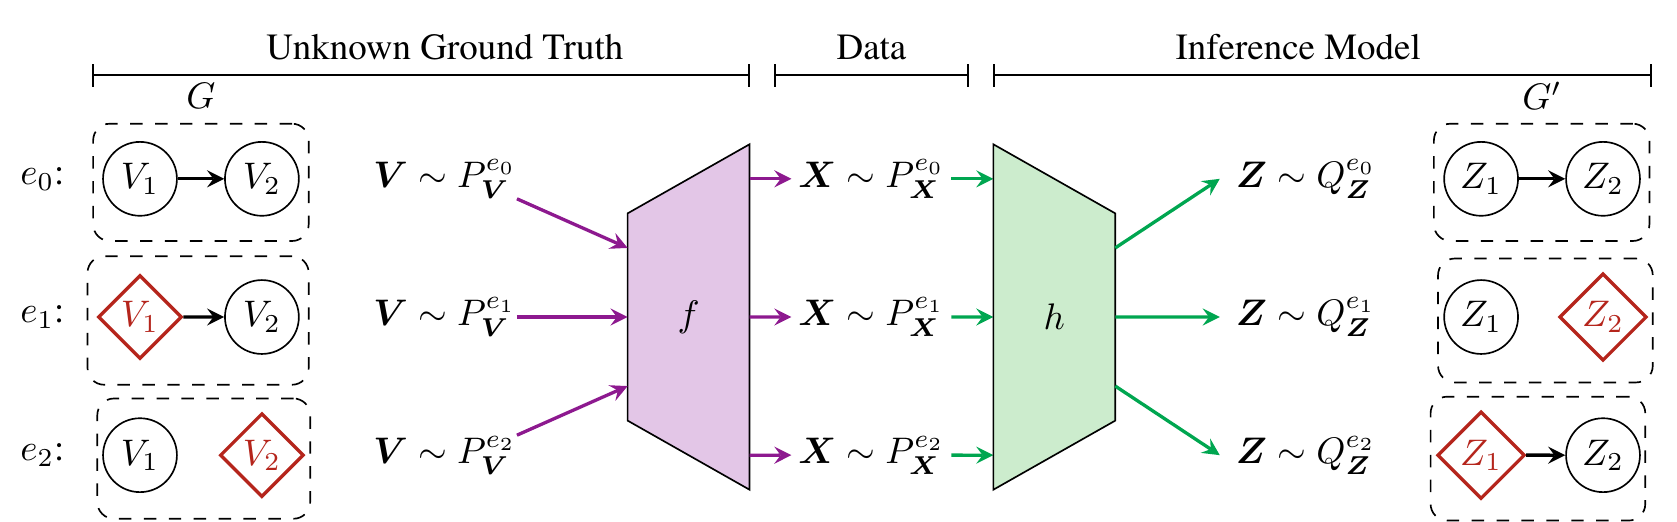
\includegraphics[width=0.8\textwidth]{figures/vk_fig2}
	\begin{itemize}
		\item The model may explain environment $e_1$ as an intervention on the \emph{other} latent.
		\item With known targets, or with parametric models, this case does not arise. It is the technical novelty of the paper.
		\item Such a wrong explanation is possible only if original and intervened mechanisms are fine-tuned to each other. Generic models exclude it, in the same spirit as faithfulness.
	\end{itemize}
	\src{Figure: von K\"ugelgen et al., 2023, Fig.\ 2 (their $V$ is our $U$).}
\end{frame}

\begin{frame}{Idea 2: why the interventions must be hard}
	\begin{columns}[onlytextwidth]
		\begin{column}{0.58\textwidth}
			Comparing environments isolates $U_1$. What about its child $U_2$?
			\begin{itemize}
				\item A wrong representation could mix the parent into the child: $Z_2 = U_2 + g(U_1)$.
				\item \textbf{Hard} intervention on $U_2$: the true $U_2$ becomes independent of $U_1$. The mixed $Z_2$ would still depend on $U_1$, so the error is visible.
				\item \textbf{Soft} intervention on $U_2$: the true $U_2$ still depends on $U_1$. The mixed $Z_2$ looks like one more valid mechanism.
			\end{itemize}
		\end{column}
		\begin{column}{0.38\textwidth}
			\centering
			\begin{tikzpicture}
				\node[lat] (a) {$U_1$}; \node[intv,right=12mm of a] (b) {$U_2$};
				\draw[gone] (a) -- (b);
				\node[lbl,right=2mm of b] {hard};
				\node[lat,below=10mm of a] (c) {$U_1$}; \node[intv,right=12mm of c] (d) {$U_2$};
				\draw[arr] (c) -- (d);
				\node[lbl,right=2mm of d] {soft};
			\end{tikzpicture}
		\end{column}
	\end{columns}
	\medskip
	\begin{block}{Take-away}
		Hard interventions cut a variable off from its causes, and this is what allows recovering each latent on its own. With soft interventions this is lost.
	\end{block}
\end{frame}

\begin{frame}{Experiment: the likelihood finds the right graph and targets}
	\centering
	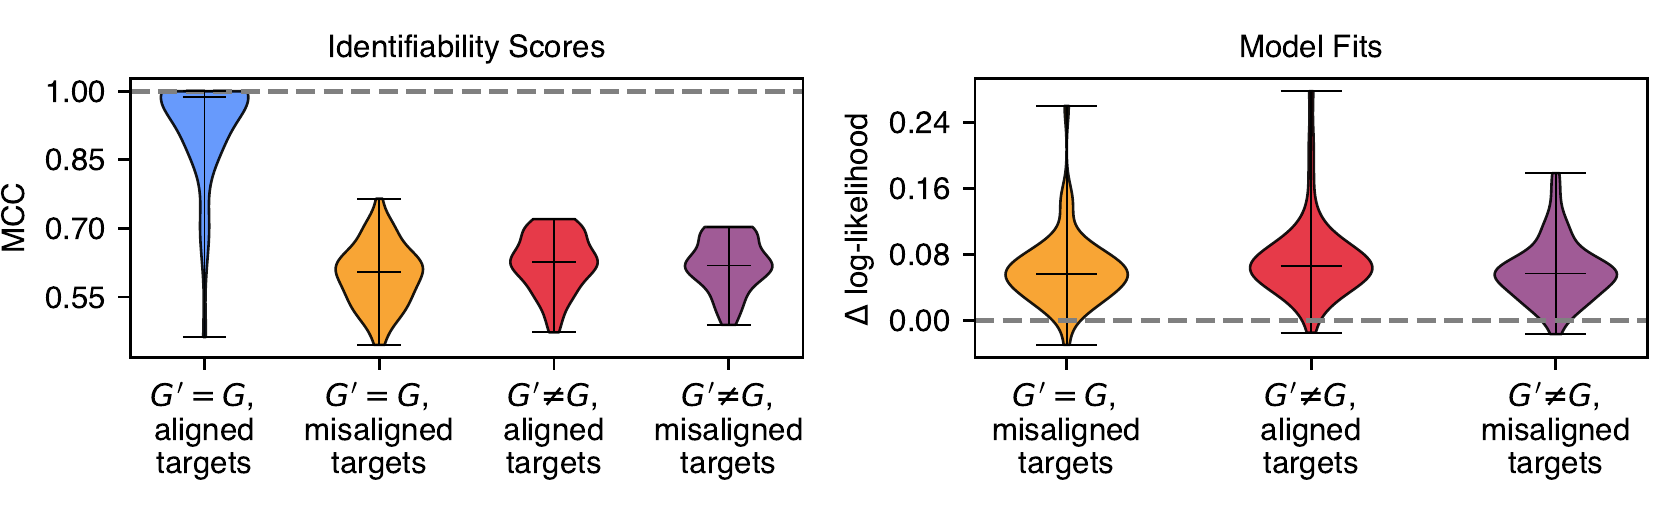
\includegraphics[width=0.8\textwidth]{figures/vk_fig3}
	\begin{columns}[onlytextwidth,t]
		\begin{column}{0.44\textwidth}
			\textbf{Setup}
			\begin{itemize}
				\item $n = 2$ latents with $U_1 \to U_2$, observations in dimension $2$.
				\item One normalizing flow per choice of graph and targets.
				\item 50 ground-truth models.
			\end{itemize}
		\end{column}
		\begin{column}{0.52\textwidth}
			\textbf{Findings}
			\begin{itemize}
				\item Right: wrong graph or targets usually gives a lower held-out likelihood.
				\item Left: only the correctly specified model recovers the latents (MCC near 1).
			\end{itemize}
		\end{column}
	\end{columns}
	\src{Figure: von K\"ugelgen et al., 2023, Fig.\ 3.}
\end{frame}

%======================================================================
\section{Limitations and motivation for the main paper \hfill {\normalsize Francesco}}
%======================================================================

\begin{frame}{Limitations of the nonparametric result}
	\begin{itemize}
		\item \textbf{Only perfect interventions.} The argument fails for soft ones, and many real perturbations are soft: CRISPR activation modulates a gene, it does not cut it off from its regulators.
		\medskip
		\item \textbf{The number of latents is assumed known.}
		\medskip
		\item \textbf{More than two latents need paired interventions} on every node.
		\medskip
		\item \textbf{No scalable algorithm.} The method fits one model per graph and per assignment of targets, which is intractable beyond a few latents.
		\medskip
		\item \textbf{Experiments are synthetic and tiny}: two or three latents.
	\end{itemize}
	\bigskip
	The paper itself points to weaker notions of identifiability for soft interventions as future work.
\end{frame}

\begin{frame}{The two papers side by side}
	\centering
	\renewcommand{\arraystretch}{1.25}
	{\scriptsize
	\begin{tabular}{@{}p{0.2\textwidth}p{0.36\textwidth}p{0.36\textwidth}@{}}
		\toprule
		& \textbf{von K\"ugelgen et al.} & \textbf{Zhang et al.\ (main paper)} \\
		\midrule
		Latent mechanisms & nonparametric & nonparametric \\
		Mixing $f$ & any smooth invertible map & \red{full-rank polynomial} (includes linear) \\
		Interventions & hard only & \red{soft}, hard included \\
		How many & $n=2$: one per node, plus observational\newline any $n$: a pair per node & at least one per node, plus observational \\
		Number of latents & assumed known & \red{identified from the data} \\
		Targets & unknown & unknown \\
		What is identified & latents up to rescaling, graph & graph and targets; effect of unseen combinations of interventions \\
		Algorithm & likelihood, search over graphs and targets & \red{discrepancy-based VAE}, gradient-based \\
		Data & synthetic, 2--3 latents & Perturb-seq, 5{,}000 genes, about 100{,}000 cells \\
		\bottomrule
	\end{tabular}}
\end{frame}

\begin{frame}{Motivation for the main paper}
	\begin{columns}[onlytextwidth,t]
		\begin{column}{0.47\textwidth}
			\begin{block}{Give up}
				\begin{itemize}
					\item A fully general mixing: $f$ is a polynomial.
					\item Recovering every latent one by one.
				\end{itemize}
			\end{block}
		\end{column}
		\begin{column}{0.47\textwidth}
			\begin{block}{Gain}
				\begin{itemize}
					\item Soft interventions.
					\item Unknown number of latents.
					\item One intervention per node for any $p$.
					\item An algorithm that runs on real genomic data.
				\end{itemize}
			\end{block}
		\end{column}
	\end{columns}
	\bigskip
	\textbf{Question for the rest of the talk:}\\[1mm]
	If interventions only \emph{change} mechanisms instead of replacing them, what can still be identified, and how do we learn it?
\end{frame}

%======================================================================
\section{Main paper: identifiability from soft interventions \hfill {\normalsize Joan}}
%======================================================================

\begin{frame}{The model: polynomial mixing, soft interventions}
	\begin{columns}[onlytextwidth,t]
		\begin{column}{0.47\textwidth}
			\begin{block}{Model}
				\begin{itemize}
					\item Latent DAG model with nonparametric mechanisms.
					\item Mixing $f$: a polynomial of $U$. Linear mixing is a special case.
					\item The number of latents $p$ is \alert{unknown}.
				\end{itemize}
			\end{block}
		\end{column}
		\begin{column}{0.47\textwidth}
			\begin{block}{Data}
				\begin{itemize}
					\item Observational data plus at least one intervention per latent.
					\item Interventions are \alert{soft}.
					\item Unpaired samples, unknown targets.
				\end{itemize}
			\end{block}
		\end{column}
	\end{columns}
	\bigskip
	\textbf{First idea: observational data already does part of the job.}
	\begin{itemize}
		\item The number of latents is the smallest dimension that can generate the data.
		\item The latents are recovered up to an unknown linear map, and no further.
		\item What remains is a linear unmixing problem, $X = U\Lambda + b$. Interventions have to solve it.
	\end{itemize}
\end{frame}

\begin{frame}{What can be recovered from soft interventions}
	\begin{columns}[onlytextwidth,t]
		\begin{column}{0.47\textwidth}
			\begin{block}{Recovered}
				\begin{itemize}
					\item Which interventions act on the same latent.
					\item The causal graph between the latents, up to their names.
					\item The effect of unseen \emph{combinations} of interventions.
				\end{itemize}
			\end{block}
		\end{column}
		\begin{column}{0.47\textwidth}
			\begin{block}{Not recovered}
				\begin{itemize}
					\item Each latent on its own.
					\item For $U_1 \to U_2$, replacing $U_2$ by $U_2 + U_1$ gives another valid model: a soft intervention never separates a variable from its parents.
				\end{itemize}
			\end{block}
		\end{column}
	\end{columns}
	\bigskip
	This is exactly the step that needed hard interventions in the first paper.\\[1mm]
	The causal structure and the predictions survive, and these are what the application needs.
\end{frame}

\begin{frame}{Linear mixing can hide a causal effect}
	\begin{columns}[onlytextwidth]
		\begin{column}{0.6\textwidth}
			With observed variables, an intervention on $U_i$ changes the marginals of its descendants. That reveals who is downstream of whom.\\[2mm]
			With mixing this is not enough (Example 1):
			\begin{itemize}
				\item Truth: $U_1 \to U_2$, with $I_1$ and $I_2$ shifting $U_1$ and $U_2$.
				\item Take $\hat U = (U_2,\ U_2 - U_1)$. It generates the same $X$.
				\item In $\hat U$ the graph is \emph{reversed}: the effect of $I_1$ on $U_2$ is cancelled in $U_2 - U_1$.
			\end{itemize}
		\end{column}
		\begin{column}{0.36\textwidth}
			\centering
			\begin{tikzpicture}
				\node[lat] (a) {$U_1$}; \node[lat,below=9mm of a] (b) {$U_2$};
				\draw[arr] (a) -- (b);
				\node[lbl,left=1mm of a,text=ETHRed] {$I_1$}; \node[lbl,left=1mm of b,text=ETHRed] {$I_2$};
				\node[lat,right=16mm of a] (c) {$\hat U_1$}; \node[lat,below=9mm of c] (d) {$\hat U_2$};
				\draw[arr,ETHRed] (d) -- (c);
				\node[lbl,right=1mm of c,text=ETHRed] {$I_1$}; \node[lbl,right=1mm of d,text=ETHRed] {$I_2$};
				\node[lbl,below=1mm of b] {truth}; \node[lbl,below=1mm of d] {same data};
			\end{tikzpicture}
		\end{column}
	\end{columns}
	\medskip
	\begin{block}{What is needed}
		The effect of an intervention must stay visible after mixing: it cannot be cancelled by linear combinations. This is faithfulness, adapted to interventions and mixing, and it holds generically.
	\end{block}
\end{frame}

\begin{frame}{Idea 1: interventions reveal who is upstream}
	\begin{columns}[onlytextwidth]
		\begin{column}{0.6\textwidth}
			\begin{itemize}
				\item An intervention changes the distribution of its target and of everything downstream, and of nothing else.
				\item A \textbf{source} node is special: its distribution changes under exactly one intervention, its own.
				\item So: search for a linear combination of $X$ whose distribution changes under one intervention only. It must be a source, and that intervention targets it.
				\item Remove the sources and repeat on the rest.
			\end{itemize}
		\end{column}
		\begin{column}{0.36\textwidth}
			\centering
			\begin{tikzpicture}[node distance=8mm and 8mm]
				\node[intv] (a) {$U_1$};
				\node[lat,below left=of a] (b) {$U_2$};
				\node[lat,below right=of a] (c) {$U_3$};
				\draw[arr] (a) -- (b); \draw[arr] (a) -- (c); \draw[arr] (b) -- (c);
				\node[lbl,above=1mm of a,text=ETHRed] {source};
			\end{tikzpicture}
		\end{column}
	\end{columns}
	\medskip
	\begin{block}{What this gives}
		The targets of all interventions and all \emph{ancestral} relations: who is upstream of whom. Not yet which edges are direct.
	\end{block}
\end{frame}

\begin{frame}{Ideas 2 and 3: the sparsest graph, and recombining mechanisms}
	\textbf{Idea 2: direct edges.}
	\begin{itemize}
		\item Many graphs share the same ancestral relations, from a chain to a complete graph.
		\item Among those compatible with the data, the true graph is the \alert{sparsest}.
	\end{itemize}
	\medskip
	\textbf{Idea 3: predicting unseen combinations.}
	\begin{itemize}
		\item Each single intervention teaches the model one changed mechanism.
		\item A combination of interventions with different targets is obtained by plugging in several changed mechanisms at once:
	\end{itemize}
	\[
		\hat U \sim \prod_{\text{not targeted}} \PP\big(\hat U_i \mid \hat U_{\pa(i)}\big) \cdot \prod_{\text{targeted}} \red{\PP^{I}\big(\hat U_i \mid \hat U_{\pa(i)}\big)}, \qquad X = \hat f(\hat U)
	\]
	The model can generate data for a double perturbation it has never seen.
\end{frame}

%======================================================================
\section{Main paper: the discrepancy-based VAE \hfill {\normalsize Joan}}
%======================================================================

\begin{frame}{From the theory to an algorithm}
	\begin{itemize}
		\item From the theory: the true graph is the sparsest model that fits all datasets.
		\item This suggests a penalized likelihood. Searching over DAGs is combinatorial, so the search is relaxed and done by gradient descent.
		\item The likelihood is replaced by a variational lower bound, as in a VAE.
	\end{itemize}
	\medskip
	\begin{block}{Re-parameterization}
		Each mechanism is written with its own independent noise: $U_i = s_i(U_{\pa(i)}, Z_i)$. With a prior $p(Z)$ and an encoder $q_\phi(Z \mid X)$,
		\[
			\log p_{\theta,\varnothing}(x) \ \geq\ \underbrace{\mathbb{E}_{q_\phi(Z \mid x)} \log p_{\theta,\varnothing}(x \mid Z)}_{\text{reconstruction}} \ \underbrace{-\, D_{\mathrm{KL}}\big(q_\phi(Z \mid x)\,\|\,p(Z)\big)}_{\text{regularization}} .
		\]
	\end{block}
	The decoder has two parts: a deep SCM from $Z$ to $U$, then the mixing $f_\theta$ from $U$ to $X$.
\end{frame}

\begin{frame}{Architecture}
	\framesubtitle{Figure: Zhang et al., 2023, Fig.\ 4}
	\begin{columns}[onlytextwidth]
		\begin{column}{0.64\textwidth}
			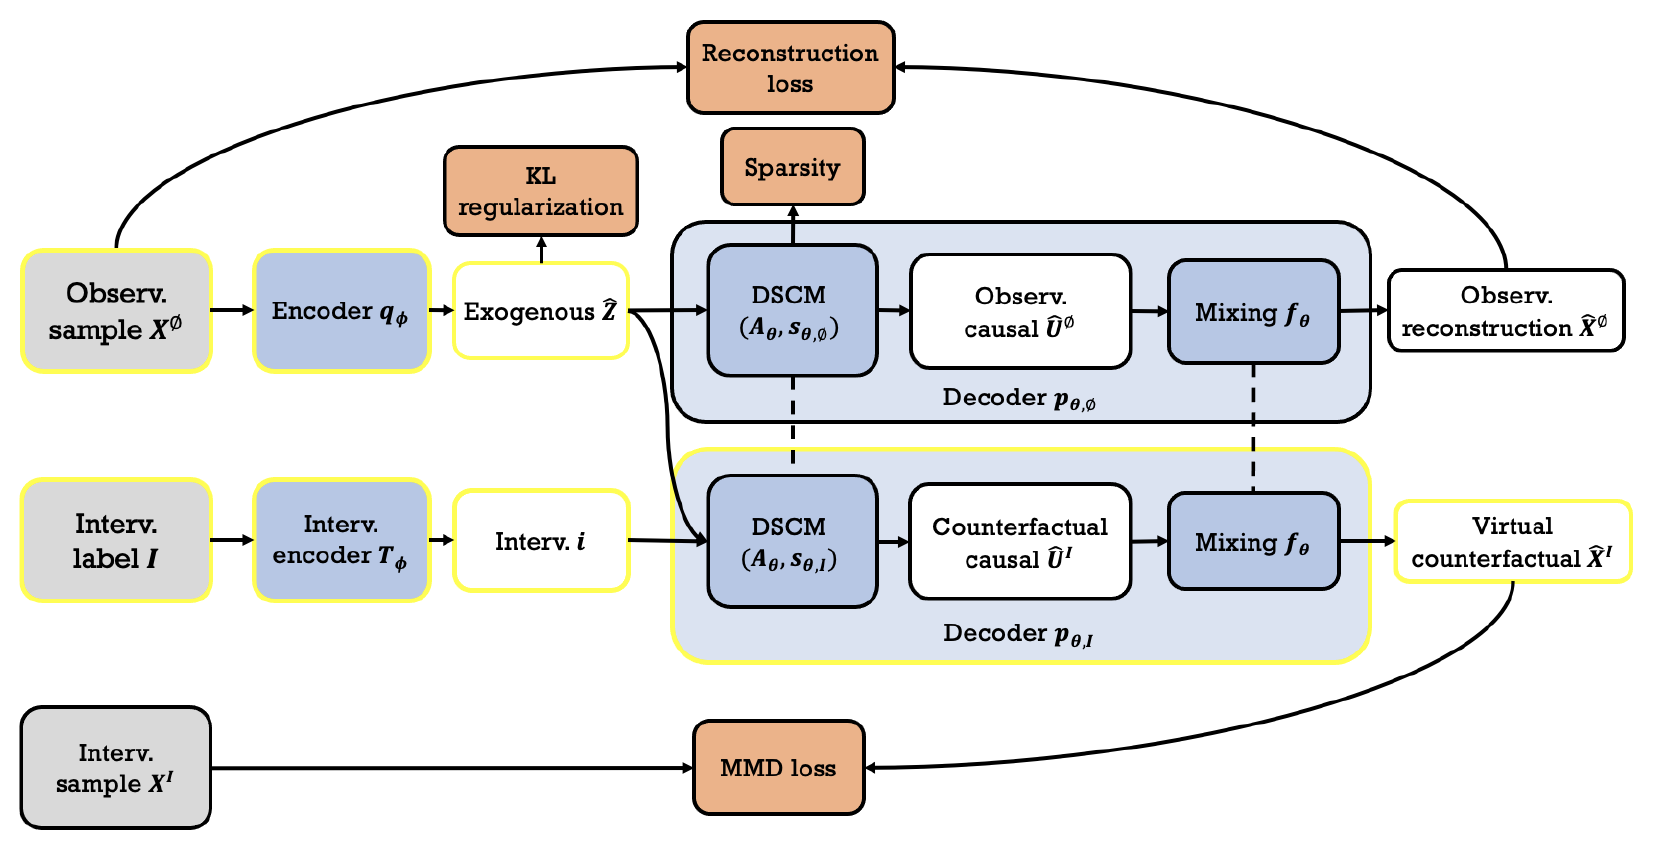
\includegraphics[width=\textwidth]{figures/zh_fig4}
		\end{column}
		\begin{column}{0.33\textwidth}
			\begin{itemize}
				\item \textbf{Top row}: a VAE on observational samples. Decoder: deep SCM with graph $A_\theta$, then mixing $f_\theta$.
				\item \textbf{Intervention encoder}: label $I$ $\mapsto$ target $i$ and shift $a_i$.
				\item \textbf{Middle row}: the same noise $\hat Z$ through the intervened SCM gives a \alert{virtual counterfactual}.
				\item \textbf{Bottom}: compare these, in distribution, with real interventional samples.
			\end{itemize}
		\end{column}
	\end{columns}
\end{frame}

\begin{frame}{The loss}
	\[
		\mathcal{L} = \mathbb{E}_{X^\varnothing}\Big[\mathcal{L}^{\mathrm{reg}}(X) + \beta\, \mathcal{L}^{\mathrm{recon}}(X)\Big] + \alpha\, \mathcal{L}^{\mathrm{discrep}} + \lambda\, \mathcal{L}^{\mathrm{sparse}}
	\]
	\begin{itemize}
		\item $\mathcal{L}^{\mathrm{discrep}} = -\sum_{k} \mathrm{MMD}\big(\text{virtual counterfactuals of } I_k,\ \D^{I_k}\big)$: the model must reproduce each interventional distribution. No pairing is needed, only a distance between two samples.
		\item $\mathcal{L}^{\mathrm{sparse}} = -\lVert A_\theta \rVert_1$: prefer the sparsest graph, as the theory asks.
		\item $A_\theta$ is upper triangular. This costs nothing, since the order of the latents is arbitrary.
		\item MMD is used instead of an adversarial distance to avoid saddle-point optimization.
	\end{itemize}
	\medskip
	\begin{block}{Guarantees}
		The loss lower-bounds the log-likelihood one would optimize with true counterfactual pairs, and the procedure is consistent: with infinite data it recovers the generative process, under suitable conditions.
	\end{block}
\end{frame}

%======================================================================
\section{Main paper: experiments and conclusion \hfill {\normalsize Joan}}
%======================================================================

\begin{frame}{Data: a large Perturb-seq screen}
	\framesubtitle{Norman et al., 2019}
	\begin{columns}[onlytextwidth,t]
		\begin{column}{0.47\textwidth}
			\begin{block}{Dataset}
				\begin{itemize}
					\item 8{,}907 unperturbed cells.
					\item 99{,}590 perturbed cells.
					\item CRISPR activation of one or two out of 105 genes: $K = 217$ interventions.
					\item Each cell: expression of 5{,}000 highly variable genes.
				\end{itemize}
			\end{block}
		\end{column}
		\begin{column}{0.47\textwidth}
			\begin{block}{Protocol}
				\begin{itemize}
					\item Latent dimension $p = 105$.
					\item Train on unperturbed cells and the 105 single-gene interventions.
					\item Hold out 96 cells for each single-gene intervention with more than 800 cells.
					\item All 112 double-gene interventions are held out \emph{entirely}.
				\end{itemize}
			\end{block}
		\end{column}
	\end{columns}
	\bigskip
	CRISPR activation is modelled as a shift intervention.
\end{frame}

\begin{frame}{Single-gene interventions}
	\centering
	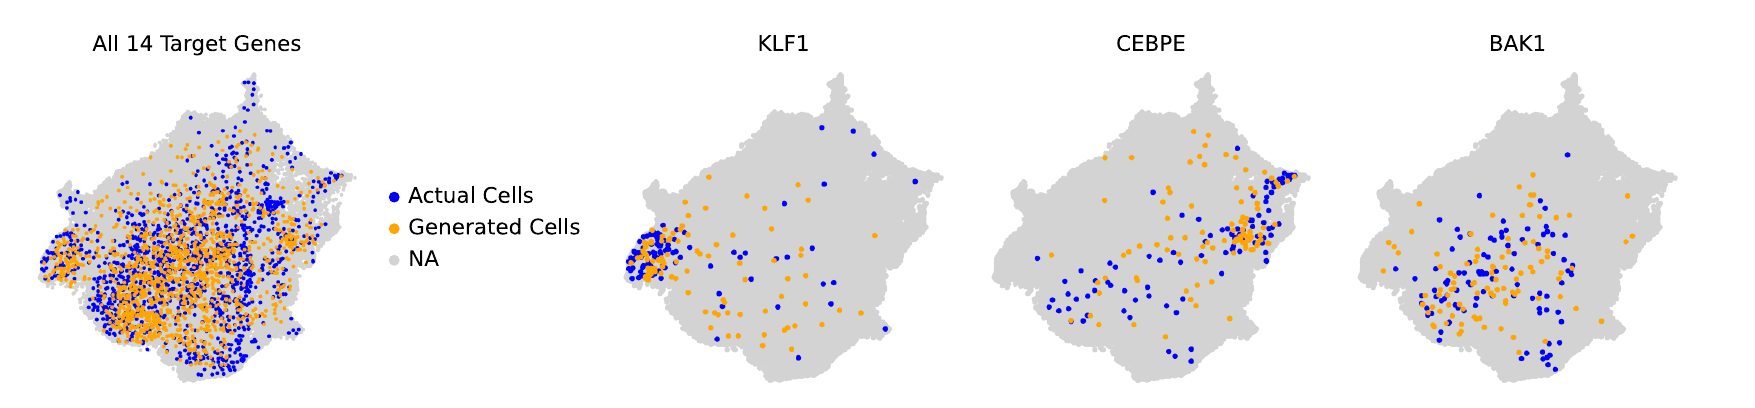
\includegraphics[width=0.86\textwidth]{figures/zh_fig5}
	\begin{columns}[onlytextwidth]
		\begin{column}{0.56\textwidth}
			\begin{itemize}
				\item Generated cells fall in the same regions as held-out real cells (UMAP).
				\item The model finds the subpopulation specific to each perturbation, e.g.\ KLF1.
				\item $R^2$ is $0.99$ on average over all genes, and $0.95$ on the 20 most differentially expressed genes.
			\end{itemize}
		\end{column}
		\begin{column}{0.4\textwidth}
			\centering
			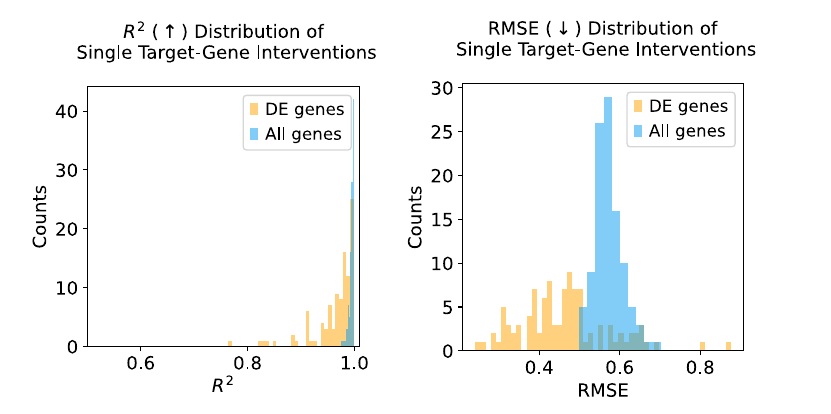
\includegraphics[width=\textwidth]{figures/zh_fig6}
		\end{column}
	\end{columns}
	\src{Figures: Zhang et al., 2023, Fig.\ 5 and 6.}
\end{frame}

\begin{frame}{Unseen double interventions and the learned graph}
	\begin{columns}[onlytextwidth]
		\begin{column}{0.4\textwidth}
			\textbf{Double-gene interventions, never seen in training}
			\begin{itemize}
				\item $R^2 = 0.98$ over all genes, $0.88$ on the most differentially expressed ones.
				\item Some pairs are predicted poorly. A possible reason: the two genes act non-additively.
			\end{itemize}
			\medskip
			\textbf{Structure learning}
			\begin{itemize}
				\item $p$ is reduced until every latent is targeted: $p = 7$ gene programs.
				\item The learned edges DUSP9 $\to$ MAPK1 and DUSP9 $\to$ ETS2 agree with Norman et al.
			\end{itemize}
		\end{column}
		\begin{column}{0.58\textwidth}
			\centering
			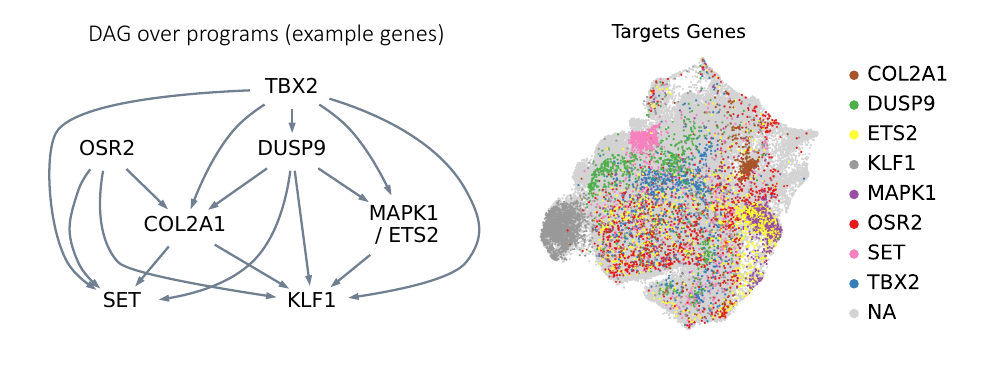
\includegraphics[width=\textwidth]{figures/zh_fig7}
		\end{column}
	\end{columns}
	\src{Figure: Zhang et al., 2023, Fig.\ 7.}
\end{frame}

\begin{frame}{Conclusion}
	\begin{columns}[onlytextwidth,t]
		\begin{column}{0.47\textwidth}
			\begin{block}{Takeaways}
				\begin{itemize}
					\item Observational data never identifies a latent causal model; interventions can.
					\item With no parametric assumption, hard interventions identify latents and graph.
					\item With polynomial mixing, soft interventions identify the graph and targets, and allow predicting unseen combinations.
					\item The discrepancy VAE turns this into a method that works on real perturbation data.
				\end{itemize}
			\end{block}
		\end{column}
		\begin{column}{0.47\textwidth}
			\begin{block}{Limitations of the main paper}
				\begin{itemize}
					\item An intervention on \emph{every} latent is needed. This is already partial knowledge of the latents, and it is not always feasible.
					\item Single-node interventions: drugs often hit several targets.
					\item Guarantees hold for infinite data; no sample complexity.
					\item Learning the DAG by gradient descent is sensitive to initialization.
				\end{itemize}
			\end{block}
		\end{column}
	\end{columns}
\end{frame}

\begin{closingframe}
	\vspace{15mm}
	{\Large Thank you. Questions?}

	\bigskip
	\footnotesize
	J.\ Zhang, C.\ Squires, K.\ Greenewald, A.\ Srivastava, K.\ Shanmugam, C.\ Uhler.
	\emph{Identifiability Guarantees for Causal Disentanglement from Soft Interventions.} arXiv:2307.06250, 2023.

	\medskip
	J.\ von K\"ugelgen, M.\ Besserve, L.\ Wendong, L.\ Gresele, A.\ Keki\'c, E.\ Bareinboim, D.\ M.\ Blei, B.\ Sch\"olkopf.
	\emph{Nonparametric Identifiability of Causal Representations from Unknown Interventions.} arXiv:2306.00542, 2023.
\end{closingframe}

\end{document}
